\section{Tutoriales de las aplicaciones
Android}\label{tutoriales-de-las-aplicaciones-android}

\subsection{BrujulaCompass}\label{brujulacompass}

Para realizar esta aplicación se ha tomado como base la brújula de la
\emph{ROM} MIUI. Se le ha añadido el reconocimiento de voz (\emph{ASR})
y se modificó la la interfaz de la brújula para que mostrara hacia donde
tiene que dirigirse el usuario en función del comando de voz. Veamos la
primera pantalla:

\subsubsection{Inicio de la
aplicación}\label{inicio-de-la-aplicaciuxf3n}

\begin{figure}[htbp]
\centering
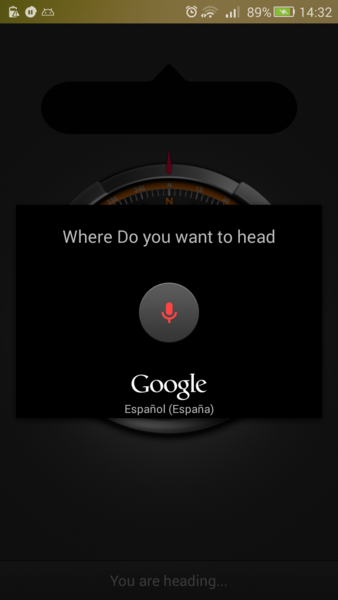
\includegraphics{./img/inicioBrujula.png}
\caption{Primera pantalla de la aplicación brújula}
\end{figure}

Al mostrarse esta pantalla, el usuario debe proporcionar un comando de
voz, por ejemplo \emph{``Norte 10''}. Tras dar el comando, en la brujula
se añadirá un marcador indicando dónde está el Norte + 10 grados. Además
de esto, mediante una voz, se le irá indicando al usuario si debe girar
a la derecha/izquierda o va en la dirección correcta:

\begin{figure}[htbp]
\centering
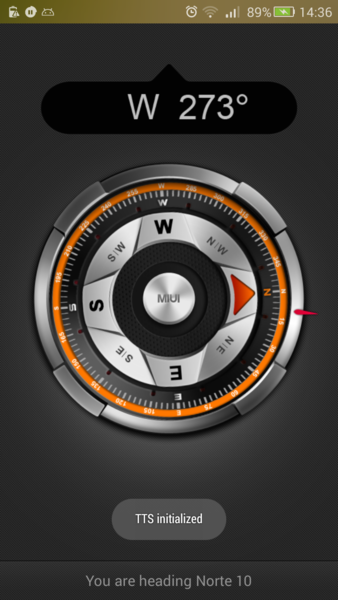
\includegraphics{./img/norte10.png}
\caption{Indicaciones en la brujula}
\end{figure}

Como vemos en la imagen, aparece un indicador rojo situado en el norte +
10 grados. Veamos otro ejemplo, Norte 45:

\begin{figure}[htbp]
\centering
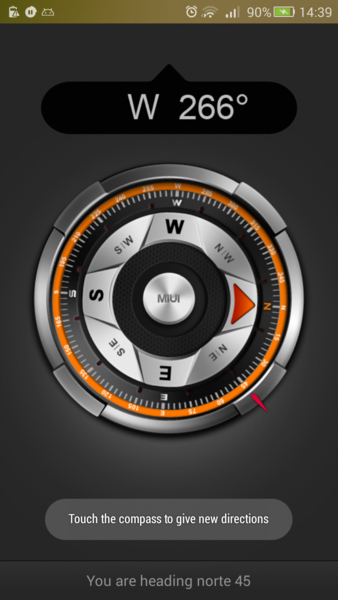
\includegraphics{./img/norte45.png}
\caption{Indicaciones en la brujula}
\end{figure}

Para dar nuevas instrucciones de voz basta con tocar la brújula.

En la parte inferior de la pantalla, aparece el comando de voz
reconocido.
